\section{Foundations of Survival Analysis}

Survival analysis comprises a rich collection of statistical methods specifically designed to analyze time-to-event data \parencite{kleinbaum2012}. As introduced in previous chapters, these methods address scenarios where the primary interest is the timing of events rather than just whether they occur \parencite{cox1972}. This chapter provides a comprehensive overview of the mathematical foundations and core concepts that underpin both traditional and modern survival analysis approaches.

\begin{notebox}[title=Chapter Overview]
This chapter covers:
\begin{itemize}
    \item Core mathematical functions in survival analysis and their relationships
    \item Types and properties of hazard functions
    \item Statistical handling of censored observations
    \item Likelihood construction for survival data
    \item Non-parametric estimation approaches
    \item Semi-parametric modeling with Cox proportional hazards
    \item Competing risks methodologies
    \item Limitations of classical methods
\end{itemize}
\end{notebox}

Understanding these foundations is crucial for properly interpreting results and developing innovative approaches to survival analysis, particularly when working with complex real-world datasets and modern machine learning techniques.

\section{Mathematical Framework of Survival Analysis}

Survival analysis is built upon a set of interrelated mathematical functions that provide different perspectives on time-to-event processes. Each function offers unique insights, but they are all mathematically connected, forming a coherent framework for analysis.

\subsection{Core Functions and Their Definitions}

Let $T$ be a non-negative random variable representing the time until an event of interest occurs. The distribution of $T$ can be characterized by several equivalent functions:

\begin{definitionbox}[title=Survival Function]
The \textbf{survival function}, denoted $S(t)$, represents the probability that the event has not occurred by time $t$:
\begin{equation}
    S(t) = P(T > t)
\end{equation}

Key properties:
\begin{itemize}
    \item $S(0) = 1$ (all subjects event-free at the start)
    \item $\lim_{t \to \infty} S(t) = 0$ (eventually all subjects experience the event)
    \item $S(t)$ is monotonically decreasing (risk never decreases with time)
    \item $S(t)$ is right-continuous
\end{itemize}
\end{definitionbox}

The survival function provides a direct measure of the proportion of subjects who remain event-free over time, making it particularly useful for visualization and communicating results to non-specialists.

\begin{definitionbox}[title=Cumulative Distribution Function]
The \textbf{cumulative distribution function (CDF)}, denoted $F(t)$, represents the probability that the event has occurred by time $t$:
\begin{equation}
    F(t) = P(T \leq t) = 1 - S(t)
\end{equation}

Key properties:
\begin{itemize}
    \item $F(0) = 0$ (no events at the start)
    \item $\lim_{t \to \infty} F(t) = 1$ (eventually all subjects experience the event)
    \item $F(t)$ is monotonically increasing
    \item $F(t)$ is right-continuous
\end{itemize}
\end{definitionbox}

While the CDF is the standard representation for random variables in probability theory, survival analysis often focuses on the survival function instead, as it directly captures the concept of "surviving" beyond a specific time point.

\begin{definitionbox}[title=Probability Density Function]
The \textbf{probability density function (PDF)}, denoted $f(t)$, represents the instantaneous rate of event occurrence at exactly time $t$:
\begin{equation}
    f(t) = \frac{d}{dt}F(t) = -\frac{d}{dt}S(t)
\end{equation}

Key properties:
\begin{itemize}
    \item $f(t) \geq 0$ for all $t$
    \item $\int_0^\infty f(t)dt = 1$
    \item $P(t_1 < T \leq t_2) = \int_{t_1}^{t_2} f(t)dt$
\end{itemize}
\end{definitionbox}

The PDF represents the unconditional instantaneous probability of the event occurring at time $t$. This differs from the hazard function, which considers the conditional probability given survival to time $t$.

\begin{definitionbox}[title=Hazard Function]
The \textbf{hazard function} (also called the hazard rate, intensity function, or failure rate), denoted $h(t)$, represents the instantaneous rate of event occurrence at time $t$, given survival up to time $t$:
\begin{equation}
    h(t) = \lim_{\Delta t \to 0} \frac{P(t \leq T < t + \Delta t | T \geq t)}{\Delta t} = \frac{f(t)}{S(t)} = -\frac{d}{dt}\log S(t)
\end{equation}

Key properties:
\begin{itemize}
    \item $h(t) \geq 0$ for all $t$
    \item $h(t)$ has no upper bound (can exceed 1)
    \item The shape of $h(t)$ reveals how risk changes over time
    \item Different from a probability (represents a rate)
\end{itemize}
\end{definitionbox}

The hazard function is perhaps the most informative representation for understanding the dynamics of risk over time. It answers the question: "Given that a subject has survived to time $t$, what is the instantaneous risk of experiencing the event?"

\begin{definitionbox}[title=Cumulative Hazard Function]
The \textbf{cumulative hazard function}, denoted $H(t)$, represents the accumulated risk up to time $t$:
\begin{equation}
    H(t) = \int_0^t h(u)du = -\log S(t)
\end{equation}

Key properties:
\begin{itemize}
    \item $H(0) = 0$ (no accumulated risk at the start)
    \item $H(t)$ is monotonically increasing
    \item $H(t)$ has no upper bound
    \item $S(t) = \exp(-H(t))$
\end{itemize}
\end{definitionbox}

The cumulative hazard function is particularly useful for model estimation and comparison. It accumulates risk over time and has a direct relationship with the survival function.

\subsection{Relationships Between Survival Functions}

These core functions form an interconnected system where each function can be derived from the others. Figure \ref{fig:survival-function-relationships} illustrates the key relationships between these functions.

\begin{figure}[htbp]
    \centering
    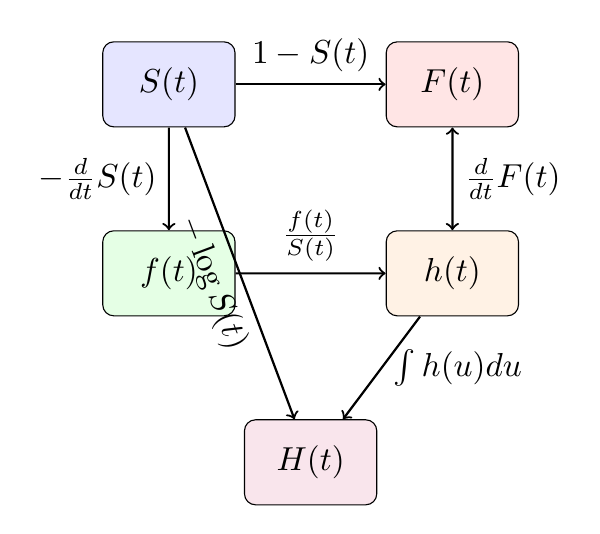
\begin{tikzpicture}[scale=1.2, transform shape]
        \node[draw, rounded corners, fill=blue!10, minimum width=1.4cm, minimum height=0.9cm] (S) at (0,0) {$S(t)$};
        \node[draw, rounded corners, fill=red!10, minimum width=1.4cm, minimum height=0.9cm] (F) at (3,0) {$F(t)$};
        \node[draw, rounded corners, fill=green!10, minimum width=1.4cm, minimum height=0.9cm] (f) at (0,-2) {$f(t)$};
        \node[draw, rounded corners, fill=orange!10, minimum width=1.4cm, minimum height=0.9cm] (h) at (3,-2) {$h(t)$};
        \node[draw, rounded corners, fill=purple!10, minimum width=1.4cm, minimum height=0.9cm] (H) at (1.5,-4) {$H(t)$};
        
        \draw[->, thick] (S) -- node[above] {$1-S(t)$} (F);
        \draw[<->, thick] (F) -- node[right] {$\frac{d}{dt}F(t)$} (h);
        \draw[->, thick] (S) -- node[left] {$-\frac{d}{dt}S(t)$} (f);
        \draw[->, thick] (S) -- node[below, sloped] {$-\log S(t)$} (H);
        \draw[->, thick] (f) -- node[above] {$\frac{f(t)}{S(t)}$} (h);
        \draw[->, thick] (h) -- node[right] {$\int h(u)du$} (H);
    \end{tikzpicture}
    \caption{Relationships between the core functions in survival analysis. Each function can be derived from the others through the transformations shown on the arrows.}
    \label{fig:survival-function-relationships}
\end{figure}

These mathematical relationships lead to several important practical formulas:

\begin{equationbox}[title=Key Mathematical Relationships]
\begin{align}
    S(t) &= \exp(-H(t)) = \exp\left(-\int_0^t h(u)du\right)\\
    f(t) &= h(t) \times S(t)\\
    h(t) &= \frac{f(t)}{S(t)} = -\frac{d}{dt}\log S(t)
\end{align}
\end{equationbox}

Understanding these relationships is crucial for model development and implementation. For example:
\begin{itemize}
    \item To derive a survival function from a specified hazard function, use $S(t) = \exp(-\int_0^t h(u)du)$
    \item To compute the density function when the hazard and survival are known, use $f(t) = h(t) \times S(t)$
    \item To estimate the hazard function from empirically derived survival estimates, use $h(t) = -\frac{d}{dt}\log S(t)$
\end{itemize}

The choice of which function to work with often depends on the specific application, computational considerations, and the specific modeling approach used.

\section{Understanding Hazard Functions}

The hazard function provides particularly valuable insights into the time-dependent risk profile. It helps identify the underlying mechanisms and patterns in time-to-event processes.

\subsection{Interpretation of the Hazard Function}

The hazard function $h(t)$ represents the instantaneous rate of failure at time $t$, given survival to time $t$. While it is not a probability (it can exceed 1), it can be interpreted as follows:

\begin{itemize}
    \item For small time intervals $\Delta t$, the quantity $h(t)\Delta t$ approximates the probability of the event occurring in the interval $(t, t+\Delta t]$, given survival to time $t$
    \item Higher values of $h(t)$ indicate greater instantaneous risk
    \item The shape of $h(t)$ over time reveals how risk evolves throughout the process
    \item Comparing hazard functions between groups shows relative risk over time
\end{itemize}

\begin{notebox}[title=Intuitive Interpretation]
While mathematically defined as a conditional rate, the hazard function can be intuitively understood as:
\begin{itemize}
    \item In medical contexts: The force of mortality or the propensity to fail at time $t$
    \item In engineering: The wear-out rate or proneness to failure at a specific point in a component's life
    \item In business: The customer's tendency to churn or cancel service at a given point in their lifecycle
\end{itemize}

The shape of the hazard function often provides clues about the underlying mechanisms driving the event process.
\end{notebox}

\subsection{Common Hazard Patterns}

Different processes exhibit characteristic hazard patterns that reflect their underlying mechanisms. Understanding these common patterns helps with model selection and interpretation.

\subsubsection{Constant Hazard}

The simplest hazard pattern is the constant hazard, where the instantaneous risk remains unchanged over time.

\begin{equationbox}[title=Constant Hazard Function]
\begin{equation}
    h(t) = \lambda \quad \text{for all } t \geq 0
\end{equation}

where $\lambda > 0$ is a constant rate parameter.

This leads to:
\begin{align}
    H(t) &= \lambda t\\
    S(t) &= \exp(-\lambda t)\\
    f(t) &= \lambda \exp(-\lambda t)
\end{align}
\end{equationbox}

\begin{figure}[htbp]
    \centering
    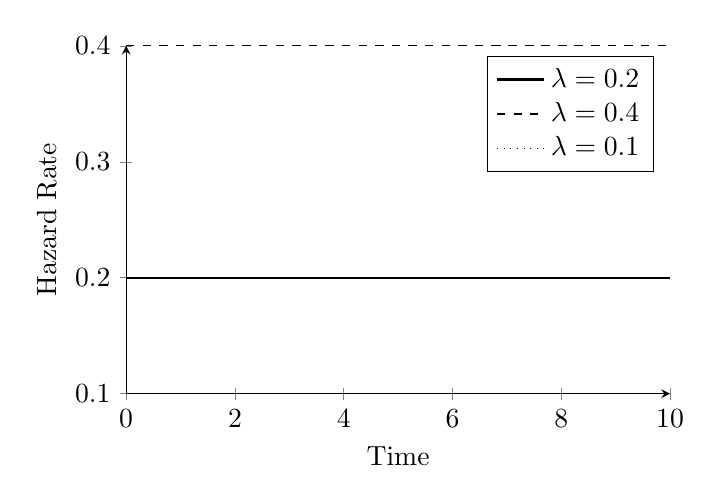
\begin{tikzpicture}
        \begin{axis}[
            width=0.7\textwidth,
            height=6cm,
            xlabel={Time},
            ylabel={Hazard Rate},
            axis lines=left,
            domain=0:10,
            samples=100,
            legend pos=north east,
          ]
          % Constant hazard (exponential)
          \addplot[black, thick] {0.2};
          \addplot[black, dashed] {0.4};
          \addplot[black, dotted] {0.1};
          \legend{$\lambda = 0.2$, $\lambda = 0.4$, $\lambda = 0.1$}
        \end{axis}
    \end{tikzpicture}
    \caption{Constant hazard functions with different rate parameters $\lambda$. A constant hazard indicates that the instantaneous risk remains stable over time, regardless of how long the subject has survived.}
    \label{fig:constant-hazard-rates}
\end{figure}

A constant hazard results in an exponential distribution for the event times. This distribution has the "memoryless" property, meaning that the future risk is independent of the past survival history.

\begin{examplebox}[title=Applications of Constant Hazard Models]
Constant hazard patterns are commonly observed in:
\begin{itemize}
    \item Random electronic component failures during their useful life period
    \item Occurrence of accidents unrelated to age or wear
    \item Events driven by random environmental factors
    \item Radioactive decay processes
    \item Some chronic disease mortality in middle age ranges
\end{itemize}

The constant hazard assumption is often used as a baseline or null model against which to compare more complex hazard patterns.
\end{examplebox}

\subsubsection{Monotonically Increasing Hazard}

Many real-world processes show increasing risk over time, reflecting aging, wear, or accumulating damage.

\begin{equationbox}[title=Weibull Increasing Hazard]
A flexible model for increasing hazard is the Weibull distribution with shape parameter $k > 1$:
\begin{equation}
    h(t) = \frac{k}{\lambda}\left(\frac{t}{\lambda}\right)^{k-1}
\end{equation}

where $k > 1$ is the shape parameter and $\lambda > 0$ is the scale parameter.
\end{equationbox}

\begin{figure}[htbp]
    \centering
    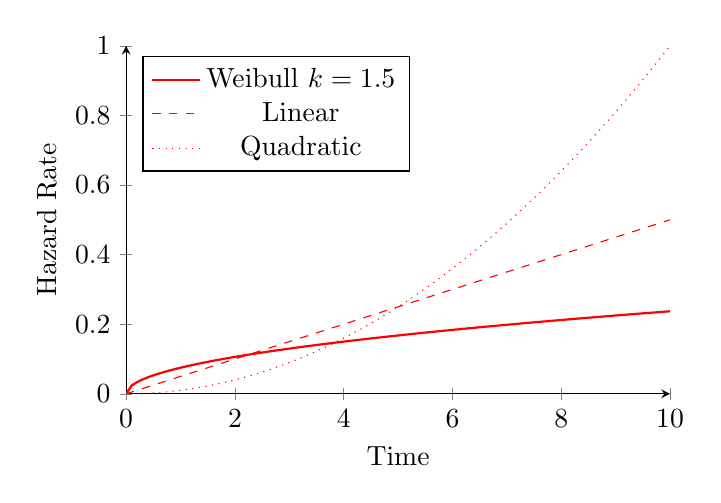
\begin{tikzpicture}
        \begin{axis}[
            width=0.7\textwidth,
            height=6cm,
            xlabel={Time},
            ylabel={Hazard Rate},
            axis lines=left,
            domain=0:10,
            samples=100,
            legend pos=north west,
          ]
          % Increasing hazards with different parameters
          \addplot[red, thick] {0.075*x^0.5};
          \addplot[red, dashed] {0.05*x^1.0};
          \addplot[red, dotted] {0.01*x^2.0};
          \legend{Weibull $k=1.5$, Linear, Quadratic}
        \end{axis}
    \end{tikzpicture}
    \caption{Monotonically increasing hazard functions. These patterns indicate that risk increases with time, which is characteristic of aging, wear-out, and progressive deterioration processes.}
    \label{fig:increasing-hazard}
\end{figure}

Increasing hazards are particularly common in:
\begin{itemize}
    \item Aging processes in living organisms
    \item Mechanical wear and fatigue failures
    \item Progressive diseases where condition worsens over time
    \item Cancer recurrence risk after initial treatment
    \item Systems with cumulative damage
\end{itemize}

The rate of increase in the hazard reflects the speed of deterioration or aging in the underlying process.

\subsubsection{Monotonically Decreasing Hazard}

Some processes exhibit decreasing risk over time, often reflecting initial vulnerability followed by increasing stability.

\begin{equationbox}[title=Weibull Decreasing Hazard]
The Weibull distribution with shape parameter $k < 1$ produces a decreasing hazard:
\begin{equation}
    h(t) = \frac{k}{\lambda}\left(\frac{t}{\lambda}\right)^{k-1}
\end{equation}

where $0 < k < 1$ is the shape parameter and $\lambda > 0$ is the scale parameter.
\end{equationbox}

\begin{figure}[htbp]
    \centering
    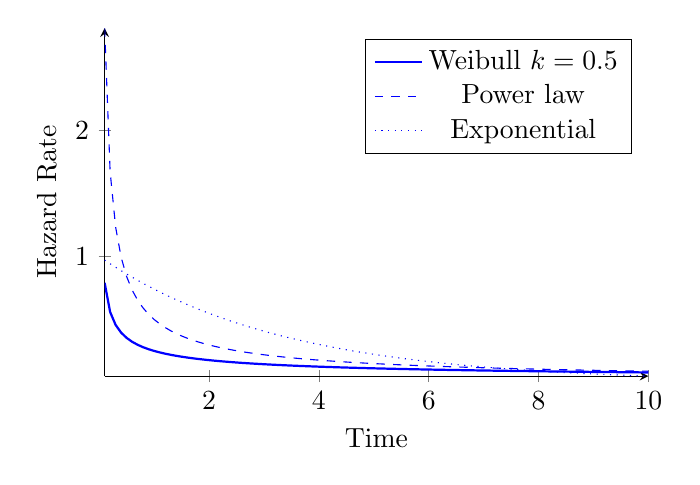
\begin{tikzpicture}
        \begin{axis}[
            width=0.7\textwidth,
            height=6cm,
            xlabel={Time},
            ylabel={Hazard Rate},
            axis lines=left,
            domain=0.1:10,
            samples=100,
            legend pos=north east,
          ]
          % Decreasing hazards with different parameters
          \addplot[blue, thick] {0.25*x^(-0.5)};
          \addplot[blue, dashed] {0.5*x^(-0.75)};
          \addplot[blue, dotted] {1.0*exp(-0.3*x)};
          \legend{Weibull $k=0.5$, Power law, Exponential}
        \end{axis}
    \end{tikzpicture}
    \caption{Monotonically decreasing hazard functions. These patterns show risk diminishing with time, which can indicate early vulnerability followed by strengthening or stabilization.}
    \label{fig:decreasing-hazard}
\end{figure}

Decreasing hazards appear in:
\begin{itemize}
    \item Infant mortality in humans and early failure in manufacturing
    \item Post-surgical infection risk, which is highest immediately after surgery
    \item Treatment efficacy that diminishes over time
    \item Immune response development after exposure
    \item Systems that strengthen or stabilize with time
\end{itemize}

Decreasing hazards often reflect selection processes where weaker subjects fail early, leaving a progressively more robust population.

\subsubsection{Non-Monotonic Hazard Patterns}

Many real-world processes exhibit more complex hazard patterns that combine elements of increasing and decreasing hazards.

\paragraph{Bathtub-Shaped Hazard}

The bathtub-shaped hazard curve starts high, decreases to a relatively stable level, and then increases again at later times.

\begin{figure}[htbp]
    \centering
    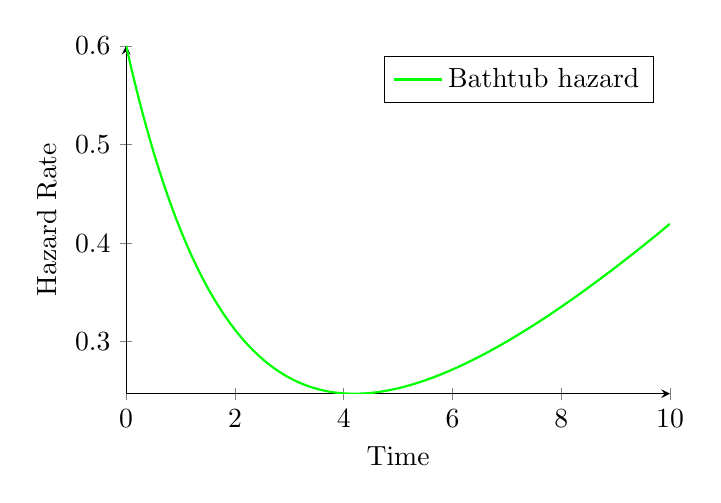
\begin{tikzpicture}
        \begin{axis}[
            width=0.7\textwidth,
            height=6cm,
            xlabel={Time},
            ylabel={Hazard Rate},
            axis lines=left,
            domain=0:10,
            samples=100,
            legend pos=north east,
          ]
          % Bathtub hazard
          \addplot[green, thick] {0.5*exp(-0.5*x) + 0.1 + 0.01*x^(1.5)};
          \legend{Bathtub hazard}
        \end{axis}
    \end{tikzpicture}
    \caption{Bathtub-shaped hazard function showing high initial risk, followed by a period of relative stability, and ending with increasing risk. This pattern is common in human mortality and complex system lifecycles.}
    \label{fig:bathtub-hazard}
\end{figure}

This pattern commonly appears in:
\begin{itemize}
    \item Human mortality across the lifespan (infant mortality, stable adulthood, aging)
    \item Complete product lifecycles (early defects, useful life, wear-out)
    \item Systems with multiple failure modes operating at different time scales
\end{itemize}

\paragraph{Hump-Shaped Hazard}

Hump-shaped (or unimodal) hazards start low, increase to a peak, and then decrease again.

\begin{figure}[htbp]
    \centering
    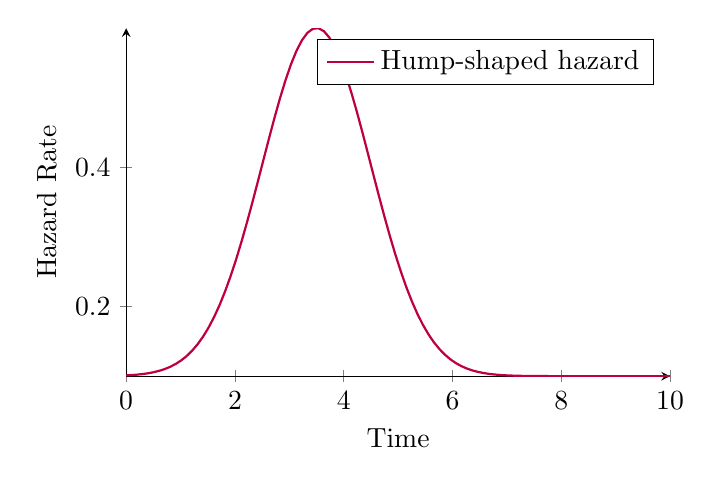
\begin{tikzpicture}
        \begin{axis}[
            width=0.7\textwidth,
            height=6cm,
            xlabel={Time},
            ylabel={Hazard Rate},
            axis lines=left,
            domain=0:10,
            samples=100,
            legend pos=north east,
          ]
          % Hump-shaped hazard
          \addplot[purple, thick] {0.1 + 0.5*exp(-(x-3.5)^2/2)};
          \legend{Hump-shaped hazard}
        \end{axis}
    \end{tikzpicture}
    \caption{Hump-shaped hazard function showing risk that increases to a peak and then decreases. This pattern often occurs in scenarios with a critical time window of vulnerability.}
    \label{fig:hump-hazard}
\end{figure}

This pattern is common in:
\begin{itemize}
    \item Post-surgical complications that peak during a critical recovery phase
    \item Treatment response patterns with a window of vulnerability
    \item Certain diseases with age-specific incidence peaks
    \item Log-normal failure distributions
\end{itemize}

\subsection{Hazard Patterns in Real-World Applications}

Recognizing hazard patterns in real data helps identify appropriate models and understand underlying mechanisms.

\subsubsection{Medical Applications}

Different medical conditions exhibit characteristic hazard patterns:
\begin{itemize}
    \item \textbf{Cancer progression:} Often shows increasing hazard as the disease advances and becomes more aggressive
    \item \textbf{Post-surgery recovery:} Typically shows high initial risk from complications, followed by declining risk
    \item \textbf{Infectious diseases:} May show hump-shaped hazards with peak risk during specific phases
    \item \textbf{Chronic conditions:} Often exhibit slowly increasing hazards reflecting progressive nature
\end{itemize}

\subsubsection{Engineering Applications}

Mechanical and electronic systems often follow well-established hazard patterns:
\begin{itemize}
    \item \textbf{Electronic components:} Often follow the bathtub curve with three distinct phases:
    \begin{itemize}
        \item Early failures due to manufacturing defects (decreasing hazard)
        \item Random failures during useful life (constant hazard)
        \item Wear-out failures in later life (increasing hazard)
    \end{itemize}
    \item \textbf{Mechanical systems:} Frequently show increasing hazards due to wear, fatigue, or corrosion
    \item \textbf{Complex systems:} May exhibit mixture patterns reflecting multiple components and failure modes
\end{itemize}

\begin{notebox}[title=Implications for Modeling]
Understanding the hazard pattern of a process provides crucial guidance for model selection:
\begin{itemize}
    \item Constant hazard processes are well-modeled by exponential distributions
    \item Monotonically changing hazards often fit well with Weibull distributions
    \item Non-monotonic hazards may require mixture models or more flexible parametric forms
    \item Complex patterns might benefit from non-parametric or semi-parametric approaches
\end{itemize}

Misspecification of the hazard pattern can lead to poor model fit and misleading conclusions.
\end{notebox}

\section{Censoring in Survival Analysis}

Censoring—the partial observation of event times—is a defining characteristic of survival data that requires specialized analytical methods. The detailed discussion of censoring, its types, and mechanisms can be found in Chapter \ref{ch:censoring}.

\subsection{Truncation vs. Censoring}

It's important to distinguish between censoring and truncation, as they represent fundamentally different data limitations.

\begin{definitionbox}[title=Truncation]
Truncation occurs when subjects are systematically excluded from the sample based on their event times. Unlike censoring (which is partial observation), truncation means complete exclusion of certain subjects.

\begin{itemize}
    \item \textbf{Left truncation:} Subjects are only included if their event time exceeds some threshold ($T > L$)
    \item \textbf{Right truncation:} Subjects are only included if their event time is less than some threshold ($T < R$)
\end{itemize}
\end{definitionbox}

Examples of truncation include:
\begin{itemize}
    \item Studies of disease duration that recruit patients who already have the disease (left truncation)
    \item Studies based on death records, which only include those who have died (right truncation)
    \item Age-specific studies that only include subjects within certain age ranges
\end{itemize}

Truncation creates a biased sample and requires special methods to correct for the bias in estimation.

\section{Likelihood Functions for Survival Data}

The likelihood function serves as the foundation for parameter estimation in survival analysis. Due to censoring, the standard likelihood approach must be adapted to handle partially observed data.

\subsection{General Principles of Likelihood Functions}

In standard statistics, the likelihood function measures the consistency between observed data and a particular set of model parameters:

\begin{equationbox}[title=Standard Likelihood Function]
For observations $X = \{x_1, x_2, \ldots, x_n\}$ and parameters $\theta$:
\begin{equation}
    \mathcal{L}(\theta | X) = p(X | \theta) = \prod_{i=1}^{n} p(x_i | \theta)
\end{equation}

where $p(x_i | \theta)$ is the probability density function for observation $x_i$.
\end{equationbox}

Maximum likelihood estimation (MLE) seeks the parameter values that maximize this likelihood:
\begin{equation}
    \hat{\theta}_{MLE} = \arg\max_{\theta} \mathcal{L}(\theta | X)
\end{equation}

For computational convenience, we often maximize the log-likelihood instead:
\begin{equation}
    \hat{\theta}_{MLE} = \arg\max_{\theta} \log\mathcal{L}(\theta | X) = \arg\max_{\theta} \sum_{i=1}^{n} \log p(x_i | \theta)
\end{equation}

\subsection{Survival Likelihood with Censoring}

In survival analysis, we observe a mixture of exact event times and censored observations. Each type contributes differently to the likelihood.

\begin{equationbox}[title=Survival Likelihood with Right Censoring]
For a dataset with $n$ subjects, each characterized by $(y_i, \delta_i)$ where $y_i$ is the observed time and $\delta_i$ is the event indicator:
\begin{equation}
    \mathcal{L}(\theta) = \prod_{i=1}^{n} [f(y_i|\theta)]^{\delta_i} [S(y_i|\theta)]^{1-\delta_i}
\end{equation}

where:
\begin{itemize}
    \item For observed events ($\delta_i = 1$): Contribution is $f(y_i|\theta)$, the density at the exact time
    \item For censored observations ($\delta_i = 0$): Contribution is $S(y_i|\theta)$, the probability of surviving beyond the censoring time
\end{itemize}
\end{equationbox}

This formulation elegantly handles both types of observations by using the event indicator $\delta_i$ to select the appropriate term for each subject.

\begin{figure}[htbp]
    \centering
    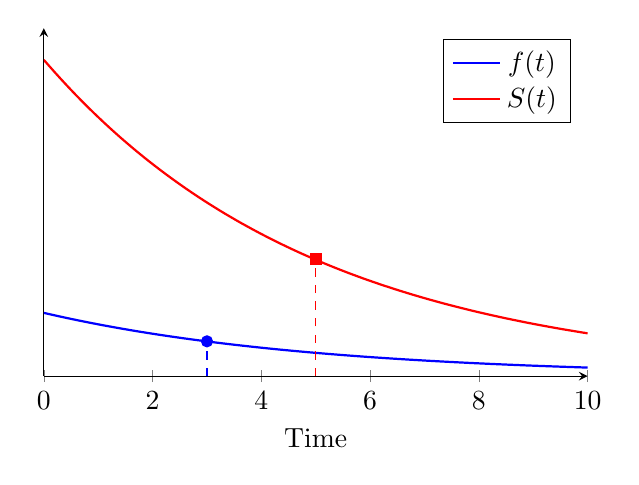
\begin{tikzpicture}
        \begin{axis}[
            width=0.7\textwidth,
            height=6cm,
            xlabel={Time},
            ylabel={},
            axis lines=left,
            domain=0:10,
            ytick=\empty,
            yticklabels={},
            ymin=0, ymax=1.1,
            legend pos=north east,
          ]
          
          % Density function
          \addplot[blue, thick, domain=0:10, samples=100] {0.2*exp(-0.2*x)};
          
          % Survival function
          \addplot[red, thick, domain=0:10, samples=100] {exp(-0.2*x)};
          
          % Observed event (use density)
          \addplot[blue, mark=*, only marks] coordinates {(3, 0.11)};
          \draw[blue, dashed] (axis cs:3,0) -- (axis cs:3,0.11);
          \node[blue] at (axis cs:3,-0.05) {$t_1$};
          
          % Censored observation (use survival)
          \addplot[red, mark=square*, only marks] coordinates {(5, 0.37)};
          \draw[red, dashed] (axis cs:5,0) -- (axis cs:5,0.37);
          \node[red] at (axis cs:5,-0.05) {$c_2$};
          
          \legend{$f(t)$,$S(t)$}
        \end{axis}
    \end{tikzpicture}
    \caption{Likelihood contributions for different observation types. For observed events (blue), the contribution is the density $f(t)$ at the exact event time. For censored observations (red), the contribution is the survival function $S(t)$ at the censoring time.}
    \label{fig:likelihood-contributions}
\end{figure}

\subsection{Alternative Formulations}

Using the relationship $f(t) = h(t)S(t)$, we can rewrite the likelihood in terms of the hazard function:

\begin{equationbox}[title=Hazard-Based Likelihood]
\begin{align}
    \mathcal{L}(\theta) &= \prod_{i=1}^{n} [h(y_i|\theta)S(y_i|\theta)]^{\delta_i} [S(y_i|\theta)]^{1-\delta_i} \\
    &= \prod_{i=1}^{n} [h(y_i|\theta)]^{\delta_i} S(y_i|\theta)
\end{align}
\end{equationbox}

Taking the logarithm and using $S(t) = \exp(-H(t))$, we obtain the log-likelihood:

\begin{equationbox}[title=Log-Likelihood for Survival Data]
\begin{align}
    \log\mathcal{L}(\theta) &= \sum_{i=1}^{n} \delta_i \log h(y_i|\theta) + \sum_{i=1}^{n} \log S(y_i|\theta) \\
    &= \sum_{i=1}^{n} \delta_i \log h(y_i|\theta) - \sum_{i=1}^{n} H(y_i|\theta)
\end{align}
\end{equationbox}

This formulation is particularly useful for model development and implementation, as it separates the components related to observed events (first term) and the risk accumulated by all subjects (second term).

\subsection{Handling Other Types of Censoring}

While the likelihood for right-censored data is most common, other types of censoring require different likelihood formulations:

\begin{itemize}
    \item \textbf{Left censoring:} For a left-censored observation at time $c$, the contribution is $F(c|\theta)$, the probability of the event occurring before time $c$
    
    \item \textbf{Interval censoring:} For an observation known to occur in the interval $(L, R)$, the contribution is $F(R|\theta) - F(L|\theta)$, the probability of the event occurring within the interval
    
    \item \textbf{Mixed censoring:} When different observations have different censoring types, each contributes appropriately according to its type
\end{itemize}

\begin{examplebox}[title=General Likelihood with Multiple Censoring Types]
For a dataset with right-censored, left-censored, and interval-censored observations:
\begin{align}
    \mathcal{L}(\theta) = \prod_{i \in \mathcal{R}} f(y_i|\theta) \prod_{j \in \mathcal{L}} F(y_j|\theta) \prod_{k \in \mathcal{I}} [F(R_k|\theta) - F(L_k|\theta)] \prod_{l \in \mathcal{C}} S(y_l|\theta)
\end{align}

where $\mathcal{R}$, $\mathcal{L}$, $\mathcal{I}$, and $\mathcal{C}$ represent the sets of exact, left-censored, interval-censored, and right-censored observations, respectively.
\end{examplebox}

\section{Non-Parametric Survival Estimation}

Non-parametric methods make minimal assumptions about the underlying distribution of survival times, providing flexible descriptive analyses of survival patterns.

\subsection{The Kaplan-Meier Estimator}

The Kaplan-Meier estimator (also called the product-limit estimator) is the most widely used non-parametric approach for estimating the survival function from right-censored data.

\begin{definitionbox}[title=Kaplan-Meier Estimator]
For a dataset with observed times $t_1 < t_2 < \cdots < t_k$, the Kaplan-Meier estimator of the survival function is:
\begin{equation}
    \hat{S}(t) = \prod_{i: t_i \leq t} \left(1 - \frac{d_i}{n_i}\right)
\end{equation}

where:
\begin{itemize}
    \item $d_i$ is the number of events at time $t_i$
    \item $n_i$ is the number of subjects at risk just before time $t_i$
    \item $\left(1 - \frac{d_i}{n_i}\right)$ represents the conditional probability of surviving through the interval containing $t_i$
\end{itemize}
\end{definitionbox}

The Kaplan-Meier estimator has several important properties:
\begin{itemize}
    \item It is a step function that decreases only at observed event times
    \item It is the non-parametric maximum likelihood estimator for the survival function
    \item It properly accounts for right-censored observations
    \item It does not require specification of the underlying distribution
\end{itemize}

\begin{figure}[htbp]
    \centering
    \begin{tikzpicture}
        \begin{axis}[
            width=0.7\textwidth,
            height=6cm,
            xlabel={Time},
            ylabel={Survival Probability},
            axis lines=left,
            xmin=0, xmax=10,
            ymin=0, ymax=1.05,
          ]
          % Kaplan-Meier step function
          \addplot[const plot, blue, thick, mark=none] coordinates {
            (0, 1.0) (1, 1.0) (1, 0.9) (2, 0.9) (2, 0.8)
            (3, 0.8) (3, 0.7) (4, 0.7) (4, 0.6) (5, 0.6)
            (5, 0.5) (6, 0.5) (6, 0.4) (7, 0.4) (7, 0.3)
            (9, 0.3) (9, 0.2) (10, 0.2)
          };
          
          % Confidence intervals
          \addplot[name path=upper, blue, opacity=0.1] coordinates {
            (0, 1.0) (1, 1.0) (1, 0.95) (2, 0.95) (2, 0.88)
            (3, 0.88) (3, 0.79) (4, 0.79) (4, 0.7) (5, 0.7)
            (5, 0.61) (6, 0.61) (6, 0.52) (7, 0.52) (7, 0.43)
            (9, 0.43) (9, 0.34) (10, 0.34)
          };
          
          \addplot[name path=lower, blue, opacity=0.1] coordinates {
            (0, 1.0) (1, 1.0) (1, 0.85) (2, 0.85) (2, 0.72)
            (3, 0.72) (3, 0.61) (4, 0.61) (4, 0.5) (5, 0.5)
            (5, 0.39) (6, 0.39) (6, 0.28) (7, 0.28) (7, 0.17)
            (9, 0.17) (9, 0.06) (10, 0.06)
          };
          
          \addplot[blue, fill opacity=0.2] fill between[of=upper and lower];
          
          % Add + marks for censored observations
          \addplot[only marks, mark=+, mark size=4pt, black] coordinates {
            (1.5, 0.9) (2.5, 0.8) (4.5, 0.6) (5.5, 0.5) (8, 0.3)
          };
        \end{axis}
    \end{tikzpicture}
    \caption{Kaplan-Meier estimate of the survival function with 95\% confidence intervals. The step function decreases only at observed event times, while + marks indicate censored observations. The confidence intervals (shaded region) widen over time as information decreases.}
    \label{fig:km-estimate-with-ci}
\end{figure}

\subsubsection{Confidence Intervals for Kaplan-Meier Estimates}

Greenwood's formula provides a variance estimator for the Kaplan-Meier estimate:

\begin{equationbox}[title=Greenwood's Formula]
\begin{equation}
    \text{Var}[\hat{S}(t)] = [\hat{S}(t)]^2 \sum_{i: t_i \leq t} \frac{d_i}{n_i(n_i-d_i)}
\end{equation}
\end{equationbox}

A 95\% confidence interval for the survival function at time $t$ can be constructed as:
\begin{equation}
    \hat{S}(t) \pm 1.96 \sqrt{\text{Var}[\hat{S}(t)]}
\end{equation}

Alternative formulations, such as the log-log transformation, are sometimes used to ensure the confidence limits remain within the range $[0, 1]$ and to improve the approximation for small samples.

\subsection{Nelson-Aalen Estimator}

While the Kaplan-Meier estimator focuses on the survival function, the Nelson-Aalen estimator provides a non-parametric estimate of the cumulative hazard function.

\begin{definitionbox}[title=Nelson-Aalen Estimator]
The Nelson-Aalen estimator of the cumulative hazard function is:
\begin{equation}
    \hat{H}(t) = \sum_{i: t_i \leq t} \frac{d_i}{n_i}
\end{equation}

where $d_i$ and $n_i$ are defined as in the Kaplan-Meier estimator.
\end{definitionbox}

The Nelson-Aalen estimator provides a basis for:
\begin{itemize}
    \item Estimating the cumulative hazard directly
    \item Examining temporal patterns in hazard rates
    \item Checking model assumptions
    \item Deriving an alternative estimator of the survival function:
    \begin{equation}
        \hat{S}_{NA}(t) = \exp(-\hat{H}(t))
    \end{equation}
\end{itemize}

\subsection{Comparing Groups with Non-Parametric Methods}

Non-parametric methods are particularly valuable for comparing survival between groups without assuming specific distributional forms.

\subsubsection{Log-Rank Test}

The log-rank test is the most widely used method for comparing two or more survival curves.

\begin{definitionbox}[title=Log-Rank Test]
The log-rank test compares observed versus expected events in each group under the null hypothesis of equal survival functions.

For $G$ groups, the test statistic is:
\begin{equation}
    \chi^2 = \sum_{j=1}^{G} \frac{(O_j - E_j)^2}{E_j}
\end{equation}

where $O_j$ is the observed number of events in group $j$, and $E_j$ is the expected number under the null hypothesis.

Under the null hypothesis, this statistic follows a chi-square distribution with $G-1$ degrees of freedom.
\end{definitionbox}

The log-rank test is most powerful for detecting differences when the hazard ratios between groups are constant over time (i.e., when the proportional hazards assumption holds).

\subsubsection{Weighted Log-Rank Tests}

Various weighted versions of the log-rank test give different emphasis to early or late differences in survival:
\begin{itemize}
    \item \textbf{Gehan-Breslow test:} Weights by the number at risk, giving more emphasis to early differences
    \item \textbf{Tarone-Ware test:} Uses square root of the number at risk as weights
    \item \textbf{Peto-Peto test:} Weights by a modified survival estimate, reducing the influence of late differences where data are sparse
\end{itemize}

\begin{figure}[htbp]
    \centering
    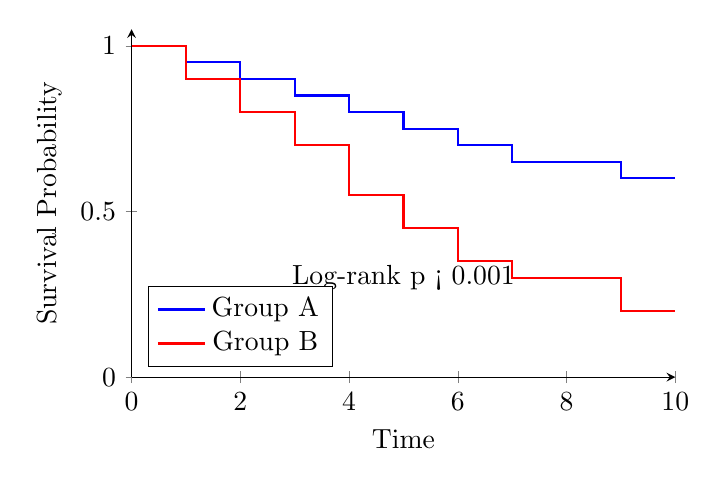
\begin{tikzpicture}
        \begin{axis}[
            width=0.7\textwidth,
            height=6cm,
            xlabel={Time},
            ylabel={Survival Probability},
            axis lines=left,
            xmin=0, xmax=10,
            ymin=0, ymax=1.05,
            legend pos=south west,
          ]
          % Group A
          \addplot[const plot, blue, thick, mark=none] coordinates {
            (0, 1.0) (1, 1.0) (1, 0.95) (2, 0.95) (2, 0.9)
            (3, 0.9) (3, 0.85) (4, 0.85) (4, 0.8) (5, 0.8)
            (5, 0.75) (6, 0.75) (6, 0.7) (7, 0.7) (7, 0.65)
            (9, 0.65) (9, 0.6) (10, 0.6)
          };
          
          % Group B
          \addplot[const plot, red, thick, mark=none] coordinates {
            (0, 1.0) (1, 1.0) (1, 0.9) (2, 0.9) (2, 0.8)
            (3, 0.8) (3, 0.7) (4, 0.7) (4, 0.55) (5, 0.55)
            (5, 0.45) (6, 0.45) (6, 0.35) (7, 0.35) (7, 0.3)
            (9, 0.3) (9, 0.2) (10, 0.2)
          };
          
          \legend{Group A, Group B}
          
          % Display p-value
          \node at (axis cs:5,0.3) {Log-rank p < 0.001};
        \end{axis}
    \end{tikzpicture}
    \caption{Kaplan-Meier curves comparing survival between two groups, with the log-rank test result indicating a significant difference.}
    \label{fig:km-comparison}
\end{figure}

\section{The Cox Proportional Hazards Model}

The Cox proportional hazards model is the most widely used approach for analyzing the effect of covariates on survival time. It represents a semi-parametric approach that balances flexibility with the ability to perform covariate adjustment.

\subsection{Model Formulation}

\begin{definitionbox}[title=Cox Proportional Hazards Model]
The Cox model specifies the hazard function for an individual with covariate vector $X$ as:
\begin{equation}
    h(t|X) = h_0(t) \exp(X\beta)
\end{equation}

where:
\begin{itemize}
    \item $h_0(t)$ is the baseline hazard function (left unspecified)
    \item $X$ is the vector of covariates
    \item $\beta$ is the vector of regression coefficients
    \item $\exp(X\beta)$ is the hazard ratio relative to baseline
\end{itemize}
\end{definitionbox}

This model has several notable features:
\begin{itemize}
    \item It makes no assumptions about the shape of the baseline hazard $h_0(t)$
    \item The effect of covariates is multiplicative on the hazard scale
    \item The hazard ratio $\exp(X\beta)$ is constant over time (the proportional hazards assumption)
    \item The log hazard is a linear function of the covariates
\end{itemize}

\subsection{Partial Likelihood Estimation}

A key innovation of the Cox model is the partial likelihood approach, which allows estimation of $\beta$ without specifying the baseline hazard $h_0(t)$.

\begin{definitionbox}[title=Partial Likelihood]
The partial likelihood for the Cox model is:
\begin{equation}
    PL(\beta) = \prod_{i: \delta_i=1} \frac{\exp(X_i\beta)}{\sum_{j \in R(t_i)}\exp(X_j\beta)}
\end{equation}

where:
\begin{itemize}
    \item The product is over observed events (not censored observations)
    \item $R(t_i)$ is the risk set at time $t_i$ (subjects still at risk just before $t_i$)
    \item The numerator represents the hazard for the subject who experienced the event
    \item The denominator sums the hazards across all subjects at risk at that time
\end{itemize}
\end{definitionbox}

The partial likelihood depends only on the order of events, not their exact timing, and eliminates the baseline hazard. Maximizing this partial likelihood yields consistent estimates of $\beta$ under the proportional hazards assumption.

\subsection{Interpretation of Parameters}

The coefficients in the Cox model have a direct hazard ratio interpretation:

\begin{examplebox}[title=Interpreting Cox Model Coefficients]
For a coefficient $\beta_j$ corresponding to covariate $X_j$:
\begin{itemize}
    \item $\exp(\beta_j)$ is the hazard ratio for a one-unit increase in $X_j$, holding other covariates constant
    \item $\beta_j > 0$ (or $\exp(\beta_j) > 1$) indicates increased hazard (worse survival)
    \item $\beta_j < 0$ (or $\exp(\beta_j) < 1$) indicates decreased hazard (better survival)
    \item $\beta_j = 0$ (or $\exp(\beta_j) = 1$) indicates no effect on hazard
\end{itemize}

Example: If $\beta_j = 0.693$ (so $\exp(\beta_j) = 2$), then a one-unit increase in $X_j$ is associated with a doubling of the hazard rate.
\end{examplebox}

\subsection{Baseline Hazard Estimation}

After estimating $\beta$, we can estimate the baseline hazard non-parametrically using the Breslow estimator:

\begin{equationbox}[title=Breslow Estimator]
\begin{equation}
    \hat{H}_0(t) = \sum_{i: t_i \leq t} \frac{d_i}{\sum_{j \in R(t_i)} \exp(X_j\hat{\beta})}
\end{equation}

where $d_i$ is the number of events at time $t_i$.
\end{equationbox}

From this, we can derive the baseline survival function:
\begin{equation}
    \hat{S}_0(t) = \exp(-\hat{H}_0(t))
\end{equation}

And the individual survival function for a subject with covariates $X$:
\begin{equation}
    \hat{S}(t|X) = [\hat{S}_0(t)]^{\exp(X\hat{\beta})}
\end{equation}

\subsection{Extensions of the Cox Model}

Several extensions address limitations of the basic Cox model:

\subsubsection{Time-Dependent Covariates}

The Cox model can accommodate covariates that change over time:
\begin{equation}
    h(t|X(t)) = h_0(t) \exp(X(t)\beta)
\end{equation}

Examples include:
\begin{itemize}
    \item Biomarkers that change during follow-up
    \item Treatment status that changes over time
    \item Environmental exposures that vary temporally
\end{itemize}

\subsubsection{Stratified Cox Model}

When the proportional hazards assumption holds within groups but not across groups, the stratified Cox model allows different baseline hazards for each stratum:
\begin{equation}
    h(t|X, s) = h_{0s}(t) \exp(X\beta)
\end{equation}

where $s$ indexes the stratum and $h_{0s}(t)$ is the stratum-specific baseline hazard.

\subsubsection{Frailty Models}

Frailty models account for unobserved heterogeneity and clustered data by introducing random effects:
\begin{equation}
    h(t|X, Z) = h_0(t) \exp(X\beta + Z)
\end{equation}

where $Z$ represents unobserved frailty (random effect) that induces correlation within clusters.

\section{Competing Risks Analysis}

Competing risks occur when subjects can experience different types of events, where the occurrence of one event precludes observation of others. A detailed discussion of competing risks can be found in Chapter \ref{ch:censoring}.

\subsection{Framework and Terminology}

In a competing risks setting, we observe:
\begin{itemize}
    \item The time to the first event: $T = \min(T_1, T_2, \ldots, T_K)$
    \item The type of the first event: $J \in \{1, 2, \ldots, K\}$
    \item Possibly right-censoring: $C$
\end{itemize}

We observe $(Y, \delta, J)$ where:
\begin{itemize}
    \item $Y = \min(T, C)$ is the observed time
    \item $\delta = I(T \leq C)$ indicates whether an event was observed
    \item $J$ indicates the type of event (when $\delta = 1$)
\end{itemize}

\subsection{Key Functions in Competing Risks}

\begin{definitionbox}[title=Cause-Specific Hazard]
The cause-specific hazard for event type $j$ is:
\begin{equation}
    h_j(t) = \lim_{\Delta t \to 0} \frac{P(t \leq T < t + \Delta t, J = j | T \geq t)}{\Delta t}
\end{equation}

This represents the instantaneous risk of event type $j$ at time $t$, given survival until time $t$.
\end{definitionbox}

\begin{definitionbox}[title=Cumulative Incidence Function]
The cumulative incidence function (CIF) for event type $j$ is:
\begin{equation}
    F_j(t) = P(T \leq t, J = j) = \int_0^t S(u) h_j(u) du
\end{equation}

where $S(t) = \exp(-\sum_{k=1}^{K}\int_0^t h_k(u)du)$ is the overall survival function.

The CIF represents the probability of experiencing event type $j$ by time $t$, accounting for the fact that other event types can occur.
\end{definitionbox}

\subsection{Modeling Approaches for Competing Risks}

Two main modeling approaches are used for competing risks:

\subsubsection{Cause-Specific Hazards Approach}

This approach models each cause-specific hazard separately, typically using Cox regression:
\begin{equation}
    h_j(t|X) = h_{0j}(t) \exp(X\beta_j)
\end{equation}

Each event type has its own baseline hazard and regression coefficients, reflecting potentially different risk factors. This approach is useful for understanding the effect of covariates on the instantaneous risk of each event type.

\subsubsection{Fine-Gray Subdistribution Hazards Approach}

The Fine-Gray approach models the subdistribution hazard directly:
\begin{equation}
    \lambda_j(t|X) = \lambda_{0j}(t) \exp(X\gamma_j)
\end{equation}

where the subdistribution hazard is defined as:
\begin{equation}
    \lambda_j(t) = \lim_{\Delta t \to 0} \frac{P(t \leq T < t + \Delta t, J = j | T \geq t \cup (T \leq t \cap J \neq j))}{\Delta t}
\end{equation}

This approach models the CIF directly and is particularly useful for risk prediction and prognostic modeling.

\begin{figure}[htbp]
    \centering
    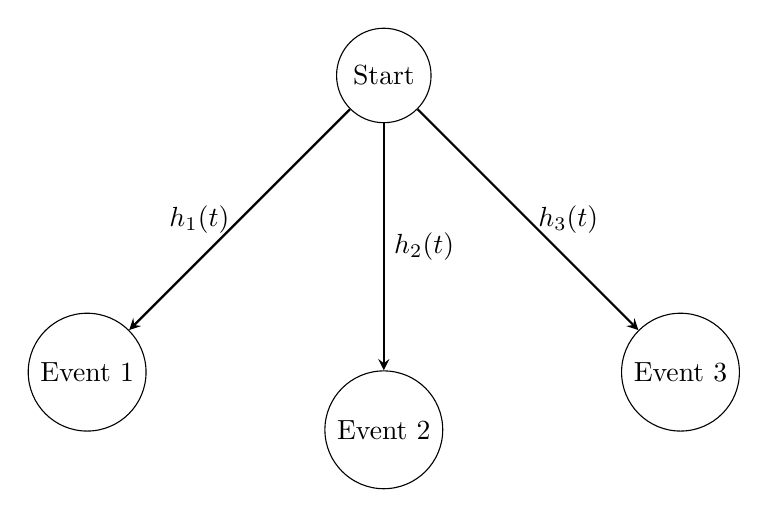
\begin{tikzpicture}[
        node distance=2.5cm,
        state/.style={circle, draw, minimum size=1.2cm},
        arrow/.style={->, >=stealth, thick}
    ]
        % States
        \node[state] (start) at (0,0) {Start};
        \node[state, below left of=start] (event1) at (-2,-2) {Event 1};
        \node[state, below of=start] (event2) at (0,-2) {Event 2};
        \node[state, below right of=start] (event3) at (2,-2) {Event 3};
        
        % Transitions
        \draw[arrow] (start) -- (event1) node[midway, left] {$h_1(t)$};
        \draw[arrow] (start) -- (event2) node[midway, right] {$h_2(t)$};
        \draw[arrow] (start) -- (event3) node[midway, right] {$h_3(t)$};
    \end{tikzpicture}
    \caption{Example of a competing risks model. From the initial state, a subject can transition to one of several possible event states, each with its own hazard function.}
    \label{fig:competing-risks-model}
\end{figure}

\section{Limitations of Classical Methods}

While classical survival analysis methods have proven invaluable across many domains, they have significant limitations, particularly for complex data and modern applications.

\subsection{Limitations of Parametric Models}

Parametric models make strong assumptions about the underlying distribution of survival times:
\begin{itemize}
    \item \textbf{Restrictive distributional assumptions:} Real-world data often do not conform to standard parametric families
    \item \textbf{Difficulty modeling complex hazard patterns:} Multi-modal or highly variable hazard shapes may not be well-approximated
    \item \textbf{Sensitivity to outliers:} Parameter estimates can be strongly influenced by extreme observations
    \item \textbf{Limited flexibility:} Fixed functional forms constrain how covariates affect survival
\end{itemize}

\subsection{Limitations of the Cox Model}

Despite its flexibility, the Cox model has several important limitations:
\begin{itemize}
    \item \textbf{Proportional hazards assumption:} The hazard ratio between any two subjects is assumed constant over time, which is often violated
    \item \textbf{Linear functional form:} Covariates are assumed to have a log-linear effect on the hazard, which may not capture complex relationships
    \item \textbf{Limited ability to model interactions:} Interactions must be pre-specified and are typically limited to low-order terms
    \item \textbf{Challenges with high-dimensional data:} The traditional Cox model is not designed for settings where the number of predictors exceeds the number of observations
\end{itemize}

\subsection{Limitations in Competing Risks Analysis}

Traditional competing risks approaches have their own challenges:
\begin{itemize}
    \item \textbf{Independence assumption:} Many methods implicitly assume independence between competing risks, which is often implausible
    \item \textbf{Difficulty modeling dependencies:} The joint distribution of event times is generally not identifiable from the observed data
    \item \textbf{Limited flexibility for risk-specific effects:} Covariates may have complex, non-linear effects that differ across event types
    \item \textbf{Challenges with time-dependent effects:} Time-varying effects are difficult to model in the competing risks framework
\end{itemize}

\subsection{The Case for Advanced Methods}

These limitations motivate the development of more flexible approaches, particularly those leveraging modern machine learning techniques:
\begin{itemize}
    \item \textbf{Capturing non-linear relationships:} Methods that can automatically detect complex patterns in data
    \item \textbf{Handling high-dimensional data:} Approaches that work well with many predictors
    \item \textbf{Modeling interactions:} Techniques that can discover interactions without explicit specification
    \item \textbf{Relaxing distributional assumptions:} Methods that make fewer assumptions about the underlying data-generating process
    \item \textbf{Incorporating time-varying effects:} Approaches that naturally accommodate changes in effects over time
\end{itemize}

\section{Modern Extensions of Classical Methods}

Building on the foundation of classical survival analysis, modern approaches incorporate advanced statistical and machine learning techniques to address many of the limitations previously discussed.

\subsection{Machine Learning Adaptations}

Several machine learning methods have been adapted for survival analysis:
\begin{itemize}
    \item \textbf{Random survival forests:} Ensemble methods that construct multiple survival trees and average their predictions, capturing non-linear effects and interactions
    \item \textbf{Survival support vector machines:} Adaptations of SVM methodology to handle censored data
    \item \textbf{Gradient boosting for survival:} Sequential construction of multiple weak learners to create a strong predictor
    \item \textbf{Neural network-based approaches:} Deep learning architectures specifically designed for time-to-event outcomes
\end{itemize}

\subsection{Flexible Modeling Approaches}

Several techniques enable more flexible modeling of survival relationships:
\begin{itemize}
    \item \textbf{Spline-based methods:} Flexible modeling of baseline hazards and time-varying effects using spline functions
    \item \textbf{Penalized methods:} Regularization approaches for high-dimensional settings
    \item \textbf{Dynamic prediction:} Methods that update predictions as new information becomes available
    \item \textbf{Joint modeling:} Simultaneous modeling of longitudinal measurements and time-to-event outcomes
\end{itemize}

\subsection{Causal Inference Methods}

Causal inference approaches bring additional rigor to survival analysis in observational settings:
\begin{itemize}
    \item \textbf{Marginal structural models:} Account for time-varying confounding through inverse probability weighting
    \item \textbf{G-computation:} Estimate causal effects through simulation of counterfactual outcomes
    \item \textbf{Instrumental variable methods for survival:} Address unmeasured confounding in survival settings
\end{itemize}

\section{Transition to Deep Learning Approaches}

The following chapters will build on these foundations to introduce modern deep learning approaches to survival analysis. These approaches combine the statistical rigor of traditional survival methods with the flexibility and power of neural networks, enabling:
\begin{itemize}
    \item Automatic feature learning from complex, high-dimensional data
    \item Capture of intricate non-linear relationships without explicit specification
    \item Integration of multiple data modalities (structured, text, images)
    \item Flexible modeling of time-varying effects
    \item Handling of competing risks and complex event patterns
\end{itemize}

\begin{notebox}[title=Looking Ahead]
In the next chapter, we will examine Deep Survival Machines (DSM), a framework that combines neural networks with mixture distribution modeling to provide flexible, interpretable survival predictions. This approach addresses many of the limitations of classical methods while maintaining the probabilistic framework necessary for valid survival analysis.
\end{notebox}

\section{Summary}

This chapter has covered the fundamental mathematical and statistical foundations of survival analysis:
\begin{itemize}
    \item The core functions that characterize time-to-event data: survival function, hazard function, and their relationships
    \item Common hazard patterns and their practical interpretations
    \item The statistical handling of censored observations through specialized likelihood functions
    \item Non-parametric approaches, particularly the Kaplan-Meier estimator
    \item The semi-parametric Cox proportional hazards model for covariate adjustment
    \item Competing risks methodology for scenarios with multiple event types
    \item Limitations of classical approaches and the motivation for modern methods
\end{itemize}

Understanding these foundations is essential for developing and applying advanced survival analysis methods. The subsequent chapters will build on this foundation to introduce deep learning approaches that retain the statistical validity of traditional methods while leveraging the flexibility and power of neural networks.